



Al fine di valutare se la scelta della tecnologia SiC-CsI può soddisfare le esigenze di NUMEN è stata implementata una simulazione Monte Carlo sulla piattaforma GEANT4.
In questo capitolo vengono esposte le principali assunzioni e vengono presentati i risultati.

\textcolor{red}{Dire che GEANT4 è basato sul C++}

%Le simulazioni giocano un ruolo fondamentale nella fisica.

%In fisica, come in altre scienze, le simulazioni giocano un ruolo fondamentale, in quanto permettono di studiare la risposta di sistemi complessi tenendo sotto controllo alcuni dei suoi gradi di libertà.

\section{\iflanguage{italian}{Le simulazioni computerizzate e i metodi Monte Carlo}{Computer simulations and Monte-Carlo methods}}


In fisica, come in altre scienze, le simulazioni computerizzate giocano un ruolo fondamentale, in quanto permettono di affrontare lo studio di sistemi che sarebbero difficilmente trattabili utilizzando tecniche teoriche o sperimentali~``classiche'';
spesso, infatti, tali approcci possono presentare problematicità legate alla complessità del sistema, al tempo necessario per lo sviluppo e l'analisi, ai costi per la realizzazione di prototipi.
Introdotte negli anni Trenta grazie all'apporto di prestigiosi scienziati come von Neumann, Ulam e Fermi, il loro progresso è stato parallelo a quello dei computer, arrivando oggi ad essere uno strumento imprescindibile in molti esperimenti.
Esse forniscono una diversa prospettiva con cui guardare alla realtà, diventando in alcuni casi una base teorica da cui partire per l'interpretazione dei risultati sperimentali, oppure in altre situazioni producendo dati ``sperimentali'' con cui mettere al vaglio le teorie.


Tra i diversi metodi di simulazione computerizzata, particolare importanza hanno assunto i cosiddetti \emph{metodi Monte Carlo}~\cite{metropolis:jasa49}, il cui nome fu coniato da Metropolis ispirandosi al casinò omonimo.
%Tali metodi utilizzano la generazione di sequenze di numeri \emph{pseudo-casuali} per simulare le fluttuazioni statistiche di un sistema con un numero elevato di gradi di libertà, 
%laddove i numeri pseudo-casuali sono dei numeri prodotti in modo deterministico ma con proprietà statistiche simili a quelle dei numeri casuali.
%
Il numero di problemi che al giorno d'oggi vengono studiati utilizzando questa tecnica è enorme, annoverando campi di ricerca estremamente diversi, che vanno dalla fisica nucleare alla fisica medica, dalla meccanica statistica alla sociofisica, dall'economia alla biologia.
%Darne una definizione comprensiva di tutte le aree di interesse è un compito difficile e sostanzialmente inutile.
%
% ***** QUESTO NON ERA MALE
%Sebbene darne una definizione comprensiva di tutte le aree di interesse sia un compito difficile, in generale è possibile dire che i metodi Monte Carlo utilizzano la generazione di numeri casuali per simulare le fluttuazioni statistiche di un sistema con un numero elevato di gradi di libertà accoppiati.
%
%
Sebbene darne una definizione comprensiva di tutte le aree di interesse sia un compito difficile, in generale è possibile dire che i metodi Monte Carlo sono dei metodi numerici di risoluzione di equazioni o di calcolo di integrali basati sulla generazione di numeri casuali.
%I metodi Monte Carlo utilizzano la generazione di numeri casuali per simulare le fluttuazioni statistiche di un sistema con un numero elevato di gradi di libertà.
Il generico metodo si compone principalmente di quattro fasi:
\begin{itemize}
	\item generazione di una sequenza di numeri casuali;
	\item calcolo delle variabili di input sulla base della sequenza estratta;
	\item determinazione delle variabili di output utilizzando le variabili di input calcolate;
	\item ripetizione dei punti precedenti e analisi critica dei risultati.
\end{itemize}



%Dal momento che i metodi Monte Carlo dipendono fortemente dalla produzione veloce ed efficiente di flussi di numeri casuali, si preferisce generare le sequenze di numeri via software, piuttosto che leggerli da tavole ad hoc.
%Tuttavia, poiché tali algoritmi sono, in realtà, deterministici, 
%In realtà, dal momento che, per ragioni di velocità ed efficienza, tali sequenze sono prodotte via software, i numeri sono \emph{pseudo-casuali}
%Per risolvere un problema complesso è necessaria una sequenza molto grande di numeri casuali, i quali devono essere indipendenti fra loro.
Affinché il metodo si dimostri efficace, è essenziale che la sequenza di numeri sia quanto più possibile casuale.
Dunque, proprio la casualità con cui vengono prodotti tali numeri rappresenta il punto più delicato del metodo e, forse, il suo limite più grande; infatti, per ragioni di velocità ed efficienza i numeri vengono generati via software, invece di basarsi su processi fisici realmente casuali.
%Tuttavia, dal momento che tali algoritmi sono inevitabilmente deterministici, le sequenze di numeri sono, in realtà, \emph{pseudo-casuali}, ovvero presentano delle proprietà statistiche simili a quelle dei numeri casuali. 
Tuttavia, dal momento che tali algoritmi sono inevitabilmente deterministici, ogni numero della sequenza è univocamente calcolato a partire dal suo predecessore. 
Quindi, le sequenze di numeri sono, in realtà, \emph{pseudo-casuali}, ovvero, pur essendo deterministiche, presentano delle proprietà statistiche analoghe a quelle delle sequenze di numeri casuali. 
Per questo motivo, una successione di numeri pseudo-casuali non può avere elementi infinitamente diversi, in quanto, prima o poi, cominceranno a ripetersi.

Negli ultimi trent'anni l'importanza delle simulazioni basate su metodi Monte Carlo è cresciuta senza soluzione di continuità. 
%Uno dei motivi di tale successo deriva in quanto al crescere della complessità del problema tale tecnica risulta superiore rispetto agli approcci analitici in termini di tempo necessario per la 
%Uno dei motivi di tale successo deriva dalla maggiore efficacia di queste tecniche rispetto agli approcci analitici nella risoluzione di problemi caratterizzati da alta complessità;
%ad esempio, valutando l'efficacia di un metodo in termini del tempo necessario per risolvere un problema, al crescere della complessità risulta che tale tempo cresce più lentamente per i metodi Monte Carlo in confronto ai metodi analitici.
%come illustrato in Figura~\ref{fig:monte_carlo}, il tempo necessario 
%Uno dei motivi di tale successo deriva dalla grande efficacia di queste tecniche nella risoluzione di problemi altamente complessi;
Una delle ragioni di tale successo deriva dalla grande efficacia di queste tecniche nell'affrontare lo studio di sistemi con un numero elevato di gradi di libertà accoppiati; 
ad esempio, è possibile dimostrare che, al crescere della complessità del problema, i metodi Monte Carlo richiedono meno tempo per giungere alla soluzione rispetto alle tecniche analitiche o deterministiche, come mostrato in Figura~\ref{fig:monte_carlo}.


\begin{figure} [!t]
	\centering
	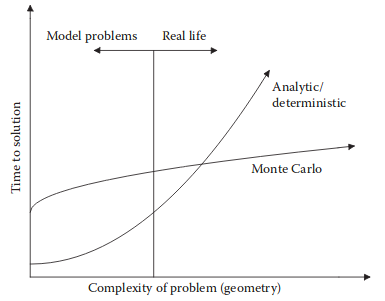
\includegraphics[scale=0.75]{Grafici/monte_carlo_vs_analytic2.png}
	\caption{Il chip VMM3 e la scheda SOM utilizzati nel test.} \label{fig:monte_carlo}
\end{figure}


%Nel campo della fisica, i metodi Monte Carlo sono spesso utilizzati per 
%Un notevole impulso allo sviluppo dei metodi Monte Carlo è provenuto dalla fisica delle alte energie, in cui l'elevata complessità degli apparati di rivelazione necessitava di uno strumento per decidere le specifiche in fase di progettazione.


Un notevole impulso allo sviluppo dei metodi Monte Carlo è provenuto dalla fisica delle alte energie, in cui la crescente necessità di simulare complessi sistemi di rivelazione spingeva per la realizzazione di software sempre più performanti e robusti.
In questo contesto nasce la piattaforma \emph{GEANT}, di cui nella sezione successiva si espongono le principali caratteristiche.





\section{\iflanguage{italian}{La piattaforma GEANT4}{GEANT4 toolkit}}


La piattaforma GEANT, il cui nome deriva da \emph{GEometry ANd Tracking}, nacque nel 1974 al CERN di Ginevra.












\clearpage


\section{\iflanguage{italian}{Gli aspetti principali della simulazione}{Simulation main aspects}}



\section{\iflanguage{italian}{I risultati}{Results}}


